\documentclass[12pt]{article}

\usepackage[utf8]{inputenc}
\usepackage[T1]{fontenc}
\usepackage{graphicx}

\title{Paralelno programiranje - 2. laboratorijska vježba}
\author{Vedran Pintarić}
\date{14. svibnja 2017.}

\begin{document}
\maketitle

\section{Uvod}
Zadatak vježbe jest implementirati igru \textit{connect 4} te implementirati
pretraživanje stanja igre uz korištenje MPI biblioteke za paralelno programiranje
tako da igrač može igrati protiv računala.

\section{Implementacija algoritma}
Prvotna implementacija pretraživanja je serijsko pretraživanje u dubinu ograničeno
na neku maksimalnu dubinu.

\subsection{Podjela}
Ideja za paralelizaciju pretraživanja u dubinu jest ta da za svako novo stanje koje
otvorimo stvaramo novi zadatak koji se može paralelno izvoditi.
U tom slučaju bi u svakoj razini
imali $W ^ d$ zadataka, gdje je $W$ širina ploče a $d$ trenutna dubina pretraživanja.

\subsection{Komunikacija}
Podaci koje procesi međusobno trebaju izmijeniti u takvoj podjeli su podaci koji opisuju
cijelo stanje koje proces treba istražiti.
Za povratnu vrijednost je potreban samo jedan broj s pomičnim zarezom.
Jedno stanje se može opisati pomoću cijelog stanja ploče, varijable koja govori tko je trenutno
na potezu te varijable koja govori koja je trenutna dubina pretraživanja.

\subsection{Aglomeracija}
Kako nije realno napraviti podjelu na način da stvaramo nove zadatke na svakoj dubini algoritma
potrebno je na drugačiji način stvarati zadatke.
Odabrana je arhitektura \textit{master - slave} gdje ce \textit{master} provesti algoritam
do neke "plitke" dubine te na toj dubini za daljnje pretraživanje stvoriti zadatke 
koje će dijeliti \textit{slave} procesima.
\textit{Slave} procesi na kraju svojeg pretraživanja vraćaju rezultat \textit{master-u} te
traže sljedeći zadatak (ako takav postoji).
Kada su svi zadaci gotovi \textit{master} može ponovno provesti svoje pretraživanje
do "plitke" dubine te sada, znajući rezultate od dubljih dubina, može provesti algoritam
do kraja te vratiti krajnje rješenje.

\subsection{Pridruživanje}
Kako je za zadatak predviđeno 8 procesora, pomoću MPI-ja možemo napraviti 1 \textit{master}
proces te maksimalno 7 \textit{slave} procesa.
Kako imamo 7 \textit{slave} procesa optimalni broj zadatak bi bio otprilike za red veličine
veći od 7.
Za širinu ploče $W = 7$ i na dubini $d = 2$ \textit{master} proces bi stvorio
$W ^ d = 49$ zadataka što nije niti previše grub ni previše fin broj zadataka za podijeliti na 7 procesa.


\section{Ispitivanje} 
Algoritam je ispitan za širinu ploče 7, visinu ploče 6 te maksimalnu dubinu pretraživanja
prostora stanja 9.
Ispitujemo algoritam uz variranje broja \textit{slave} procesa od 1 do 7.
Svaki test je proveden na pronalaženju najboljeg prvog poteza (ploča je prazna).

Prikaz trajanja algoritma za pojedini broj radnika je prikazan u tablici \ref{speed_table}.
Ubrzanja i učinkovitosti u ovisnosti o broju radnika prikazana su u grafovima \ref{speed_graph} i \ref{efficiency_graph}.

\begin{table}
\caption{Trajanje algoritma u ovisnosti o broju radnika}
\begin{center}
\begin{tabular}{ | l | c | c | c | c | c | c | c | c |}
\hline
 broj radnika & 1 & 2 & 3 & 4 & 5 & 6 & 7 & 8\\ 
\hline
 trajanje (s) & 50.15 & 27.82 & 22.62 & 20.07 & 18.30 & 15.37 & 14.68 & 14.24\\
\hline
\label{speed_table}
\end{tabular}
\end{center}
\end{table}

\begin{figure}[h]
\begin{center}
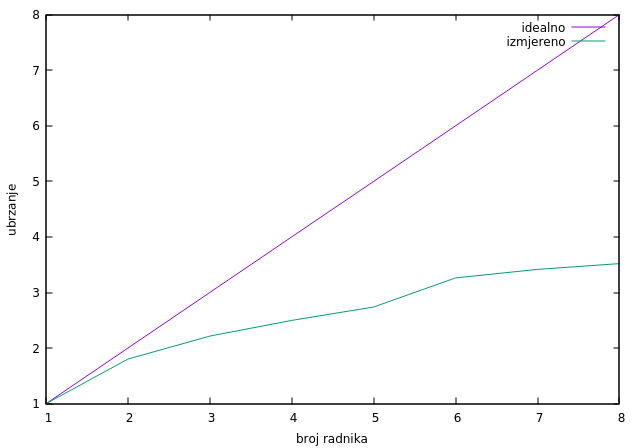
\includegraphics[width=15cm]{speed_graph}
\caption{Ubrzanje u ovisnosti broja radnika}
\label{speed_graph}
\end{center}
\end{figure}

\begin{figure}[h]
\begin{center}
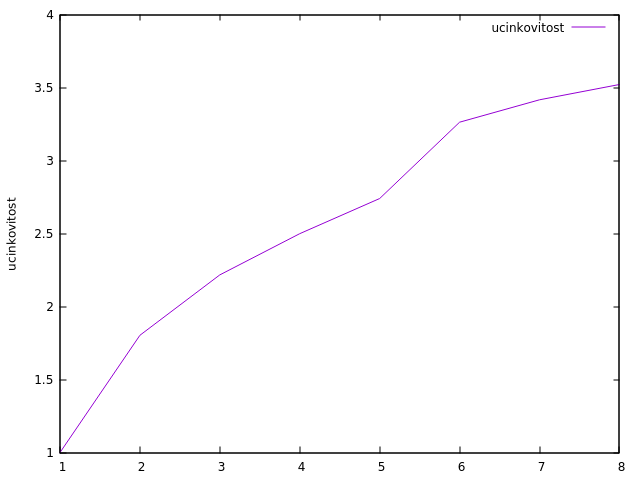
\includegraphics[width=15cm]{efficiency_graph}
\caption{Efikasnost pojedinog radnika u ovisnosti broja radnika}
\label{efficiency_graph}
\end{center}
\end{figure}

\section{Zaključak}
Zbog prilično velikih poruka koje \textit{master} proces mora slati \textit{slave} procesima
kao zadatke algoritam ne dobiva puno na ubrzanju uz veći broj \textit{slave} procesa.
Unatoč tome, paralelizacija pretraživanja se definitivno isplati za veće maksimalne dubine
gdje je veći naglasak na zadatke koje dobivaju \textit{slave} procesi nego
na poruke koje šalje \textit{master} proces.

\end{document}
  
